\documentclass[a4paper,14pt]{extarticle}
\usepackage[english,russian]{babel}
\usepackage[cache=false]{minted}
\usepackage{fontspec}
\usepackage{indentfirst}
\usepackage{listings}
\usepackage{color}
\usepackage{caption}
\usepackage{amsmath}
\usepackage{hyperref}
\usepackage{graphicx}
\usepackage[%
    left=20mm,%
    right=10mm,%
    top=20mm,%
    bottom=20mm,%
]{geometry}%
\usepackage{titlesec}


\setmainfont{PT Astra Serif}

\hypersetup{
    colorlinks=true,
    linkcolor=black,
    filecolor=magenta,
    urlcolor=cyan,
    pdftitle={Лабораторная работа №4},
    pdfpagemode=FullScreen,
}

\newcommand{\hlink}[2]{\href{#1}{\color{blue}\underline{#2}}}
\graphicspath{ {./images/} }

\setmonofont[Scale=0.8]{JetBrains Mono}
\setminted{frame=lines, framesep=3mm, fontsize=\small}
\usemintedstyle{vs}

\titleformat{\section}
{\normalfont\bfseries}{}{0pt}{Упражнение \thesection.\;}

\titleformat{\subsection}
{\normalfont\bfseries}{}{0pt}{Задание \thesubsection.\;}

\numberwithin{figure}{section}

\begin{document}

\begin{titlepage}
    \vspace{0pt plus2fill}
    \noindent

    \vspace{0pt plus6fill}
    \begin{center}
        \textbf{\large{Санкт-Петербургский национальный исследовательский университет информационных
                технологий, механики и оптики}}

        \vspace{0pt plus2fill}
        \textbf{\Large{ЛАБОРАТОРНАЯ РАБОТА №9}}

        \vspace{0pt plus2fill}
        \textbf{\large{Применение делегатов и событий}}
    \end{center}

    \vspace{0pt plus8fill}
    \begin{flushright}
        Студент: \\
        \textit{Швалов Даниил Андреевич}

        \textit{Факультет ИКТ}

        Группа: \textit{К32211}

        Преподаватель: \\
        \textit{Иванов Сергей Евгеньевич}
    \end{flushright}

    \vspace{0pt plus4fill}
    \begin{center}
        {Санкт-Петербург~--- 2023}
    \end{center}
\end{titlepage}

\section{Использование делегата при вызове метода}

В проект был добавлен класс \texttt{Operation}, который содержит статический метод \texttt{PrintTitle} для отображения информации о книге.

\inputminted{csharp}{../MyClass/MyClass/Operation.cs}

В классе \texttt{Book} был объявлен делегат \texttt{ProcessBookDelegate}, свойство \texttt{ReturnSrok}, а также метод \texttt{ProcessPaperbackBooks}.

\inputminted{csharp}{../MyClass/MyClass/Book.cs}

В класс \texttt{Program} был добавлен код для проверки программы:

\inputminted{csharp}{../MyClass/MyClass/Program.cs}

Остальные классы остались без изменений.

\inputminted{csharp}{../MyClass/MyClass/Item.cs}

\inputminted{csharp}{../MyClass/MyClass/IPubs.cs}

На рис. \ref{fig:task-1} представлен пример работы программы.

\begin{figure}[H]
    \centering
    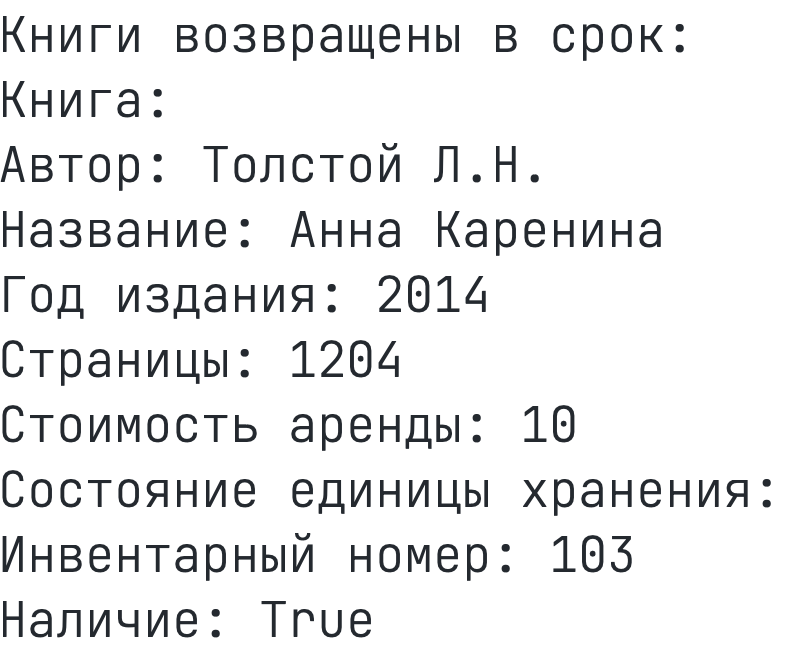
\includegraphics[width=0.5\textwidth]{images/task-1.png}
    \caption{Пример работы программы}
    \label{fig:task-1}
\end{figure}

\section{Работа с событиями}

В класс \texttt{Book} было добавлено событие \texttt{RetSrok}, изменен принцип работы свойства \texttt{ReturnSrok}, а также добавлен метод \texttt{ToString}:

\inputminted{csharp}{../MyClass1/MyClass/Book.cs}

В класс \texttt{Operation} был добавлен метод обработчик события \texttt{MetodObrabotchik}:

\inputminted{csharp}{../MyClass1/MyClass/Operation.cs}

В класс \texttt{Program} был добавлен код, проверяющий новую функциональность:

\inputminted{csharp}{../MyClass1/MyClass/Program.cs}

Все остальные классы остались без изменения:

\inputminted{csharp}{../MyClass1/MyClass/Item.cs}

\inputminted{csharp}{../MyClass1/MyClass/IPubs.cs}

На рис. \ref{fig:task-2} представлен пример работы программы.

\begin{figure}[H]
    \centering
    
\includegraphics[width=\textwidth]{images/task-2.png}
    \caption{Пример работы программы}
    \label{fig:task-2}
\end{figure}

\section{Реализация события}

В класс \texttt{IgralnayaKost} были добавлены делегат \texttt{ProcessIgralnayaKostDelegate} и событие \texttt{MaxPoints}:

\inputminted{csharp}{../Igra/IgralnayaKost.cs}

В класс \texttt{Gamer} был добавлен метод обработчик \texttt{MaxPointsHandler}. Также в конструктор была добавлена подписка на событие \texttt{MaxPoints}:

\inputminted{csharp}{../Igra/Gamer.cs}

В класс \texttt{Program} был добавлен код, проверяющий работу программы:

\inputminted{csharp}{../Igra/Program.cs}

На рис. \ref{fig:task-3} представлен пример работы программы.

\begin{figure}[H]
    \centering
    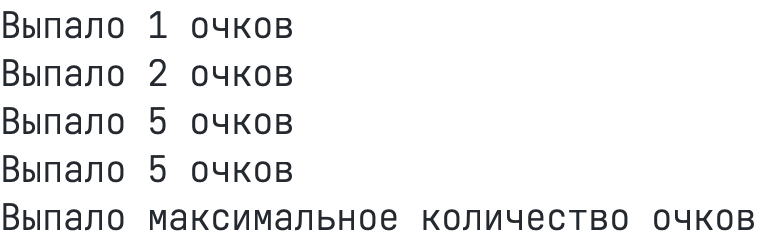
\includegraphics[width=0.5\textwidth]{images/task-3.png}
    \caption{Пример работы программы}
    \label{fig:task-3}
\end{figure}

\section{Иерархия классов учебного центра}

Абстрактный класс \texttt{Person} хранит в себе фамилию и дату рождения, а также имеет два метода: виртуальный метод \texttt{Show} и обычный метод \texttt{GetAge}:

\inputminted{csharp}{../LearningCenter/Person.cs}

Интерфейс \texttt{IEmployee} содержит метод для получения зарплаты. Этот интерфейс будет применен для реализации классов администратора, преподавателя и менеджера, т. е. сотрудников учебного центра.

\inputminted{csharp}{../LearningCenter/IEmployee.cs}

Согласно описанию, были созданы классы \texttt{Administrator}, \texttt{Student}, \texttt{Teacher} и \texttt{Manager}:

\inputminted{csharp}{../LearningCenter/Administrator.cs}

\inputminted{csharp}{../LearningCenter/Student.cs}

\inputminted{csharp}{../LearningCenter/Teacher.cs}

\inputminted{csharp}{../LearningCenter/Manager.cs}

В класс \texttt{Program} был добавлен код, проверяющий работу программу, а также выводящий список персон, возраст которых лежит в заданном пользователем диапазоне:

\inputminted{csharp}{../LearningCenter/Program.cs}

На рис. \ref{fig:task-4} представлен пример работы программы.

\begin{figure}[H]
    \centering
    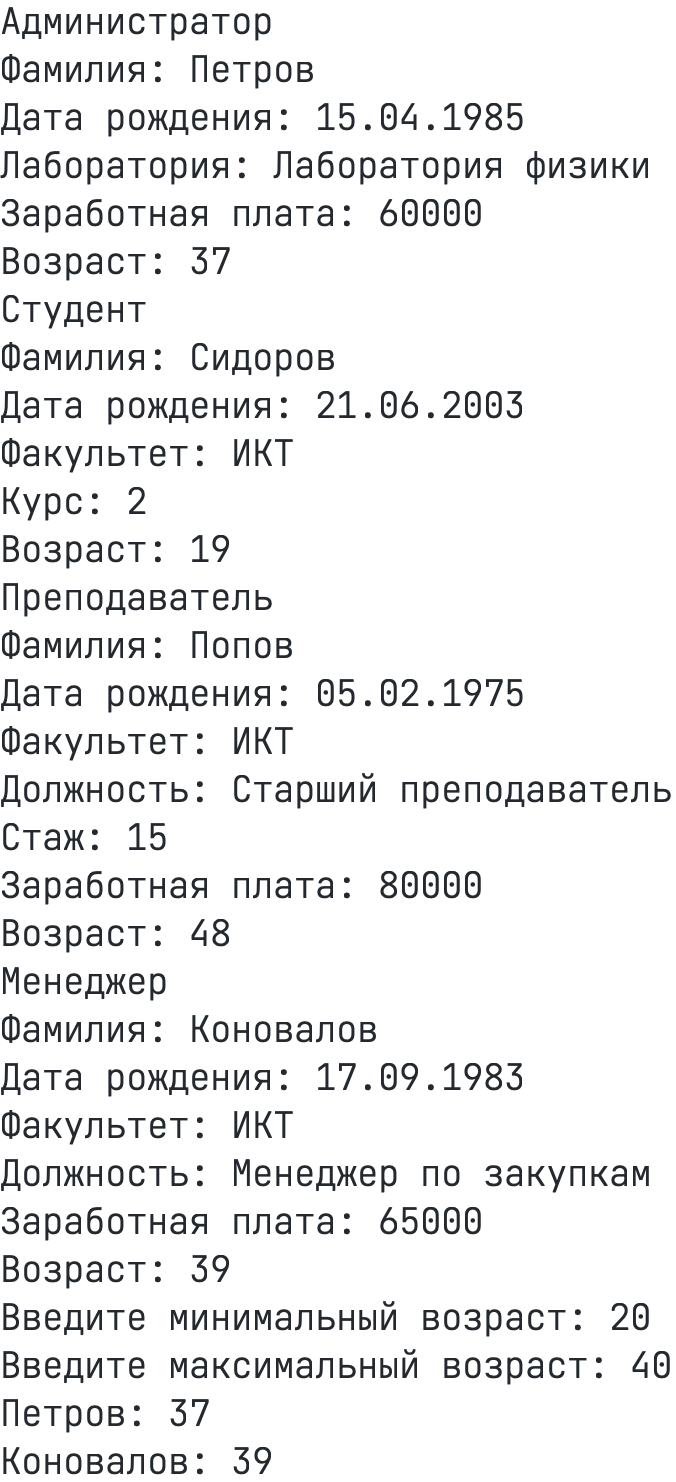
\includegraphics[width=0.5\textwidth]{images/task-4.png}
    \caption{Пример работы программы}
    \label{fig:task-4}
\end{figure}


\end{document}
